
%SPW: General: "Smith et al." are human authors.  Results are given "by" those authors, not "in" them. (Ugh!) 
% PB: fixed.


%MLNA: Sec 3 (text) needs to be much clearer as to which spectra (IRS or ISO) are being discussed.

All the main PAH features features, including the 6.2, 7.7, 8.6 and 11.3~$\mu$m bands, are clearly visible in the final processed spectra 
(see Figure \ref{PAHFITplots}) from all the regions except the nucleus. (The spectrum of the nucleus is discussed in Section 4.3.)
They also show atomic line emission such as [Ar~{\sc ii}], [Ar~{\sc iii}], [S~{\sc iii}], [S~{\sc iv}], [Ne~{\sc ii}], [Ne~{\sc iii}] 
and molecular H$_{2}$ emission at 12.3~$\mu$m. Some of the spectra display a contribution to the continuum from starlight emission.


%SPW: Sec 3 par 2: comment on NGC 206 belongs in Sec 2 and/or note to Table 1. Rest of par belongs later, when dust continuum is discussed.
Dust continuum emission from Regions 3 and 9 is very low compared to other spectra and they also show some negative flux values in the shorter 
wavelengths which can be due to instrumental errors. It was observed that the spectrum from the NGC 206 is very noisy, therefore that spectrum 
was removed from our analysis. 

%SPW: Sec 3 par 3: belongs later or perhaps omit. -- 
% PB: done?
% D : Yes. I moved it to the results section.

\subsection{ISOCAM versus IRS}
\label{sect:iso_vs_irs}

%MLNA: Sec 3.1, para 1, 1st sentence needs a reference, like maybe an ISO user's guide or some kind of technical memo.
% D : I put a reference
As mentioned in the Introduction, based on ISOCAM observations \citet{1998Cesarsky} reported a suppression of the common 
6 to 8~$\mu$m features and an enhancement of a broad 11.3 and 12.7 $\mu$m features in four regions of M31. 
In addition, \citet{Pagani_1999} confirmed that the star-forming ring in M31 shows very weak PAH emission in the 6 to 8~$\mu$m region. 
However, the IRS spectra presented here do not show such unusual behaviour (Figure \ref{PAHFITplots}). 
Indeed, except for the nucleus, all regions show a normal mid-IR spectrum similar to other nearby starforming galaxies. 
Therefore, we obtained newly-processed ISOCAM spectra from three regions in our IRS sample (see Section 2.4) % TODO: change to \ref
and compared them with the corresponding IRS spectra (Figure \ref{ISOnIRS}). 
The spectra from both instruments look almost the same. Although the relative intensities of the features in the IRS and ISOCAM 
spectra are differ in detail, the shapes of the spectra are almost identical. Except for the nucleus, there is no depletion in 
6 to 8~$\mu$m features as described by \citet{1998Cesarsky}. 
%SPW Sec 3.1 par 1: better last sentence "Figure 7 compares ...." Immediately previous reference is Sec 2.3; use \label and \ref to keep these straight.

%SPW: Sec 3.1 par 2: delete first sentence
Until 2005, ISOCAM data were not properly background subtracted and they were contaminated with zodiacal emission and stray light. 
Therefore, differential spectra between regions of relatively strong and weak emission have been used to overcome this problem 
(more details about the differential spectra are given by \citealt{1998Cesarsky}). In 2005, the ISOCAM data were reprocessed 
and corrected for the zodiacal emission \citep{Boulanger_F_2005}. For the remainder of this paper the reprocessed ISOCAM data are 
referred to as ISO2005 and earlier data as ISO1998. It is clear that the spectra obtained from these newly processed ISOCAM data 
do not agree with the previous differential spectra, especially for the bulge and the nucleus. Indeed, the differential spectrum shows a broad emission feature
around the 11.3~$\mu$m feature not visible in Figure \ref{ISOnIRS} (top). Also, the differential spectrum towards the bulge does not show 
any emission in the 6 to 8~$\mu$m region unlike the newly processed data (Figure \ref{ISOnIRS} middle).
By examining the spectra obtained from other regions  which were observed by the IRS instrument (Figure~\ref{PAHFITplots}), it can be argued that the IRS results do not support the results based on ISO1998 data.
%SPW: Sec 3.1 par 3: if you define ISOxxxx, use those designations.  Remove redundancies.  End with final sentence such as "The new reduction appears to eliminate the discrepancies." Par 4 then isn't needed.
% %(We should probably plan to send the submitted ms to Diego Cesarsky, but it's too early for that now.)




\begin{figure}
\centering
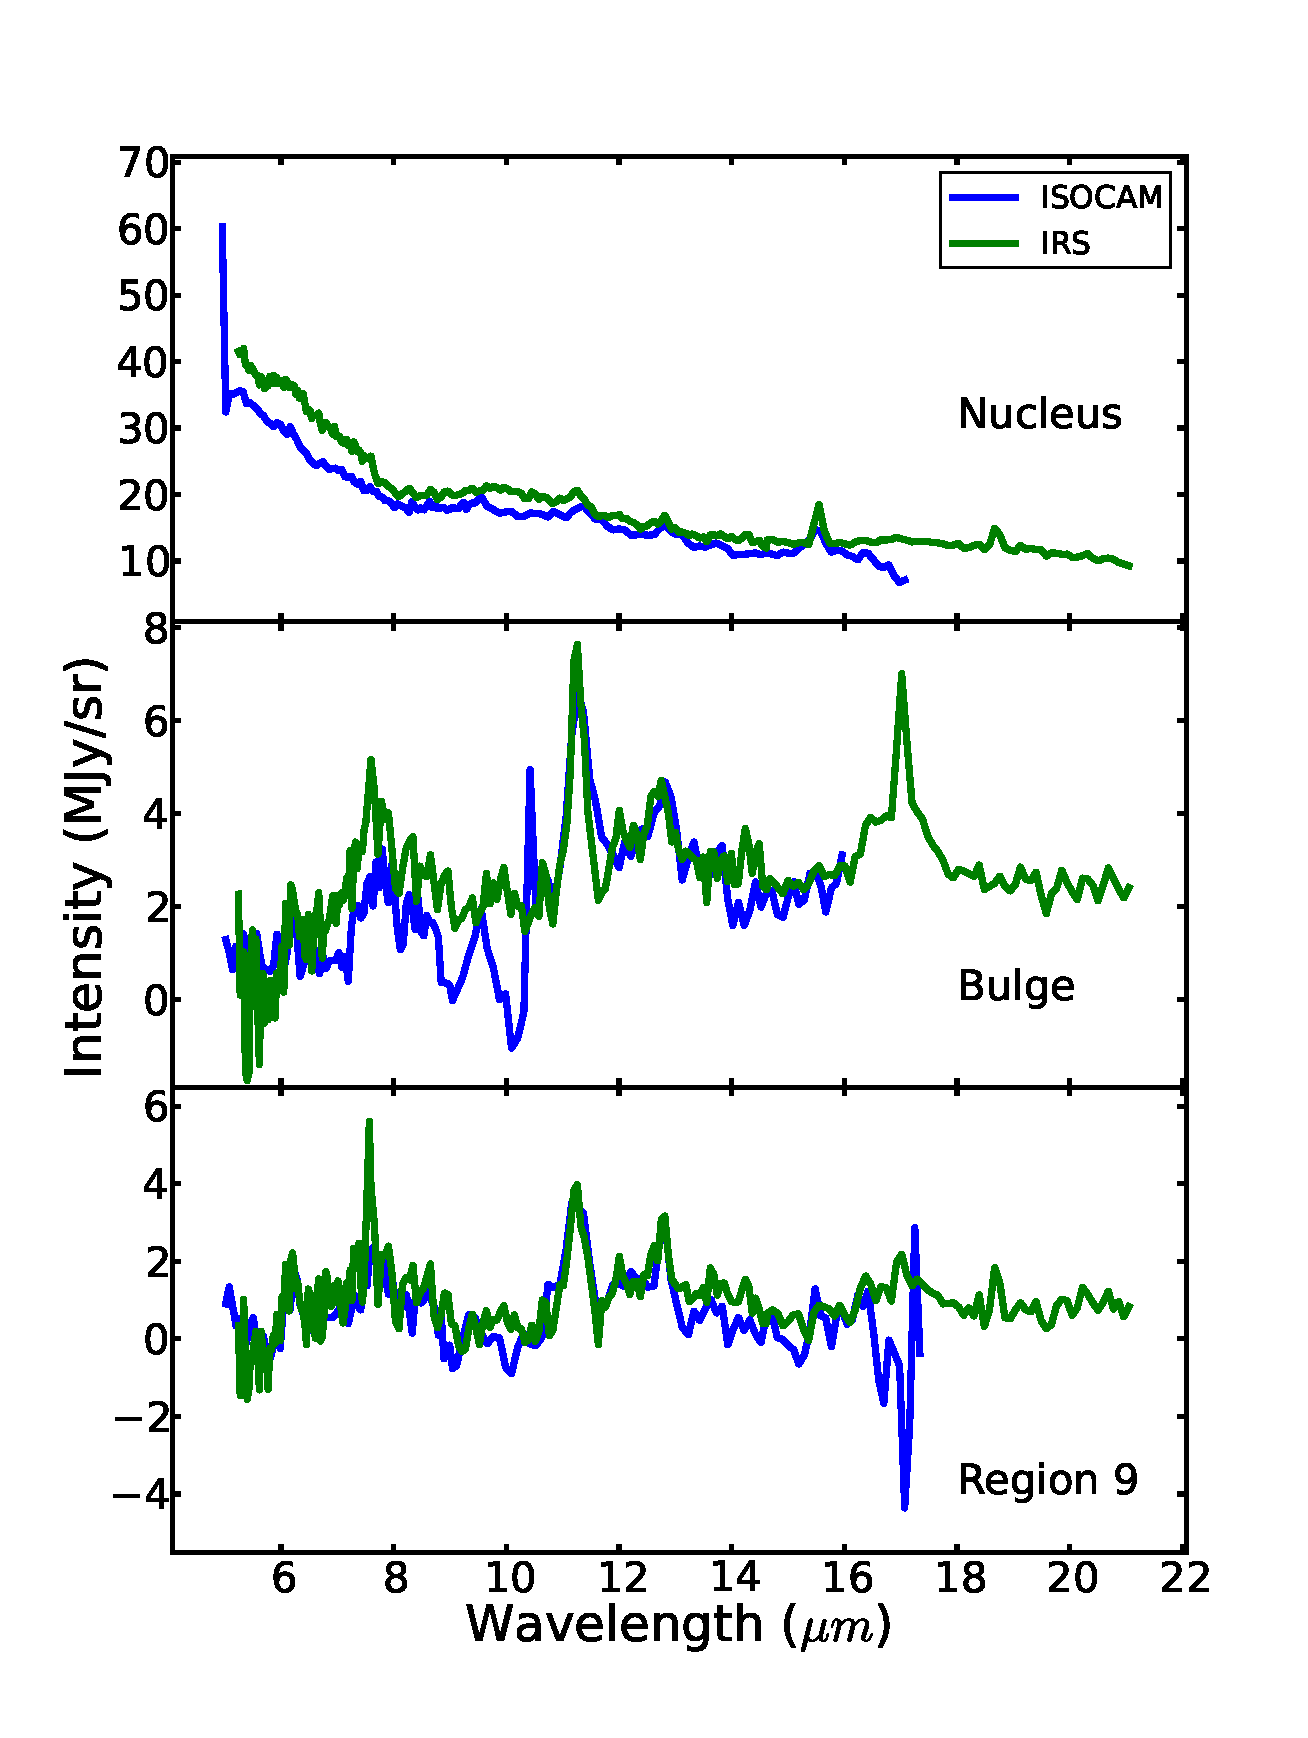
\includegraphics[scale=0.35]{./ISOvsIRS.eps}
\caption{ Comparison of  IRS and re-processed ISOCAM spectra for the Nucleus (top), Bulge (middle) and Region 9 (bottom) in M31.}
\label{ISOnIRS}
\end{figure}


\subsection{PAHFIT}

The PAH features in the IRS spectra are often blended with neighbouring aromatic features and atomic lines. Therefore measuring the strength of PAH features is difficult. To achieve this task a tool called PAHFIT, introduced by \citet{Smith:2007lr}, was used. PAHFIT is an IDL  based tool designed for decomposing {\em Spitzer} IRS spectra of PAH emission sources and is capable of identifying PAH features among other blended features. It also takes silicate absorption and extinction into account. PAHFIT is primarily designed for use with full 5--35~$\mu$m {\em Spitzer} low-resolution IRS spectra.
%SPW: Sec 3.2 par 1: I don't understand why the last sentence is needed.
%

%SPW: Sec 3.2 par 2: generally "modified blackbody" means one with an emissivity varying with wavelength.  I don't think that's what you mean for the stellar spectra.  For the dust spectra, it is likely appropriate, but the form of the variation with wavelength should be given.  I think what you mean in the middle is something like "PAHFIT uses only the minimum number of temperatures needed to fit the data, in most cases two or three for our data."  (What was the maximum number?)
PAHFIT uses six main components to fit the surface brightness. These are starlight continuum, featureless thermal dust continuum, pure rotational lines of H$_2$, fine-structure lines, dust emission features and dust extinction. The starlight is represented by a modified blackbody emission at a fixed temperature of 5000 K and the dust continuum is represented by 8 modified blackbodies at fixed temperatures of 35, 40, 50, 65, 90, 135, 200, and 300~K. However, the final fit obtained with PAHFIT does not necessarily take all dust continua into account. Line features are represented by Gaussian profiles and dust features are represented by Drude profiles. The infrared extinction is considered as a combination of a power law plus silicate features peaking at 9.7 and 18~$\mu$m. More details about PAHFIT are given by \citet{Smith:2007lr}.
%MLNA: I suppose others may know what a Drude profile is, but this is the first I've heard of it


%SPW: Sec 3.2 par 3: omit "a considerable amount of" or quantify it.  I gather the end result was forcing PAHFIT to set extinction to zero. Also starlight was zero except for the four regions. Basically this par just needs to be terser and more direct.
None of the IRS spectra shows a significant silicate absorption around 9.7 or 18~$\mu$m and the the extinction values calculated by PAHFIT were almost zero. Therefore, we adjusted the PAHFIT input parameters so that it does not take dust extinction into account. Except for the bulge, Region 5, Region 6 and Region 8, the spectra do not show much contribution from starlight. 
% MLNA: Why do you hard-wire these parameters to exclude them entirely, if there is *some* contribution seen from them in the spectra?
Therefore, the starlight parameter in PAHFIT was also set to zero so that it does not take starlight into account except for the regions mentioned above. 
PAHFIT did not fit the spectrum from the nucleus properly. This was due to the silicate emission around 9.7~$\mu$m and therefore we did not use PAHFIT data from the nucleus for our analysis.

% SPW: "Observed IRS spectra and detailed PAHFIT decompositions. Regions are labeled in each panel.  Black squares show the observed data, and ....  Vertical scales differ in different panels."  (Modify that last sentence as appropriate.)
% SPW: I'm not sure what the right-hand "Relative Extinction" scale is supposed to be, but if you keep it, explain it in the caption.
% SPW: Why are there multiple red lines (dust continuum) in some panels?
% D : PAHFIT uses multiple dust continuums 
%MLNA Figures 8 and 9 are really just the same figure, spread over two pages.  Is there any benefit to showing the fit residuals in each case?  The fits looks quite good BTW

\begin{figure*}
\centering
\includegraphics[scale=0.45]{./ALL.eps}
  \caption{The spectra from 10 regions (black squares) shown with their detailed PAHFIT decomposition. Red, blue, light blue, pink and green lines represent the dust continua, PAH features, atomic lines, starlight continuum and the fit respectively. The black line shows the total continuum. Spectra from the nucleus and NGC 206 are not shown here.}
\label{PAHFITplots}
\end{figure*}


\subsection{PAH features}
\label{sect:pah}
%SPW Sec 3.3 par 1: I'd rephrase "...coming from ordinary dust grains, much larger than PAH molecules."  Omit "Therefore ... M31."  In last sentence, do you mean regions 3 and 9?  Isn't the problem that they have negligible dust continuum, and therefore the EQWs can't be calculated? The feature flux ratios should still be meaningful, though.
%
%MLNA: Do you need to number the equation in Sec 3.3, para 1.  Also, it is unclear from the text why you write it this way instead of just putting I(nu)_feature in the numerator and then having to explain your notation in the text
PAHFIT returns fluxes and equivalent widths (EQWs) of PAH features which are given in Tables~\ref{PAHlinetable} and \ref{EQW}. The intensities of the features do not include any contribution from the continuum but the equivalent width computed by
\begin{equation}
{\rm EQW}=\int \frac{I_{\nu} - I_{\nu, {\rm cont}}}{I_{\nu, {\rm cont}}} \,d\lambda,
\end{equation}
is a measure of both the strength of the continuum emission ($I_{\nu, {\rm cont}} $) and the line strength ($I_{\nu,{\rm feature}}$). 
Here $I_{\nu} =I_{\nu,{\rm feature}}+ I_{\nu, {\rm cont}} $. 
The continuum emission is mainly coming from the dust grains. Hence, by studying EQWs of PAHs, we can study how the PAHs compete with the dust grains in the mid-IR wavelengths. Therefore the EQW values were obtained to analyze the characteristics of PAHs in M31. PAHFIT returns the EQW values for each PAH feature and the uncertainties were calculated using a Monte-Carlo method. In that method, for each region, PAHFIT was run 500 times on randomly generated data points  normally distributed within the uncertainties of the spectrum. PAHFIT returned 500 EQW values for each PAH feature and the standard deviation of EQWs for a given feature was taken as its uncertainty. 
The EQW values from Regions 3 and 9 were removed from our analysis because they have negative flux values in their spectra which can affect the EQWs. 
% TODO: change region names in above line
% D : Changed region names


\subsection{Atomic line features}
\label{sect:atomic}

\begin{figure}
\centering
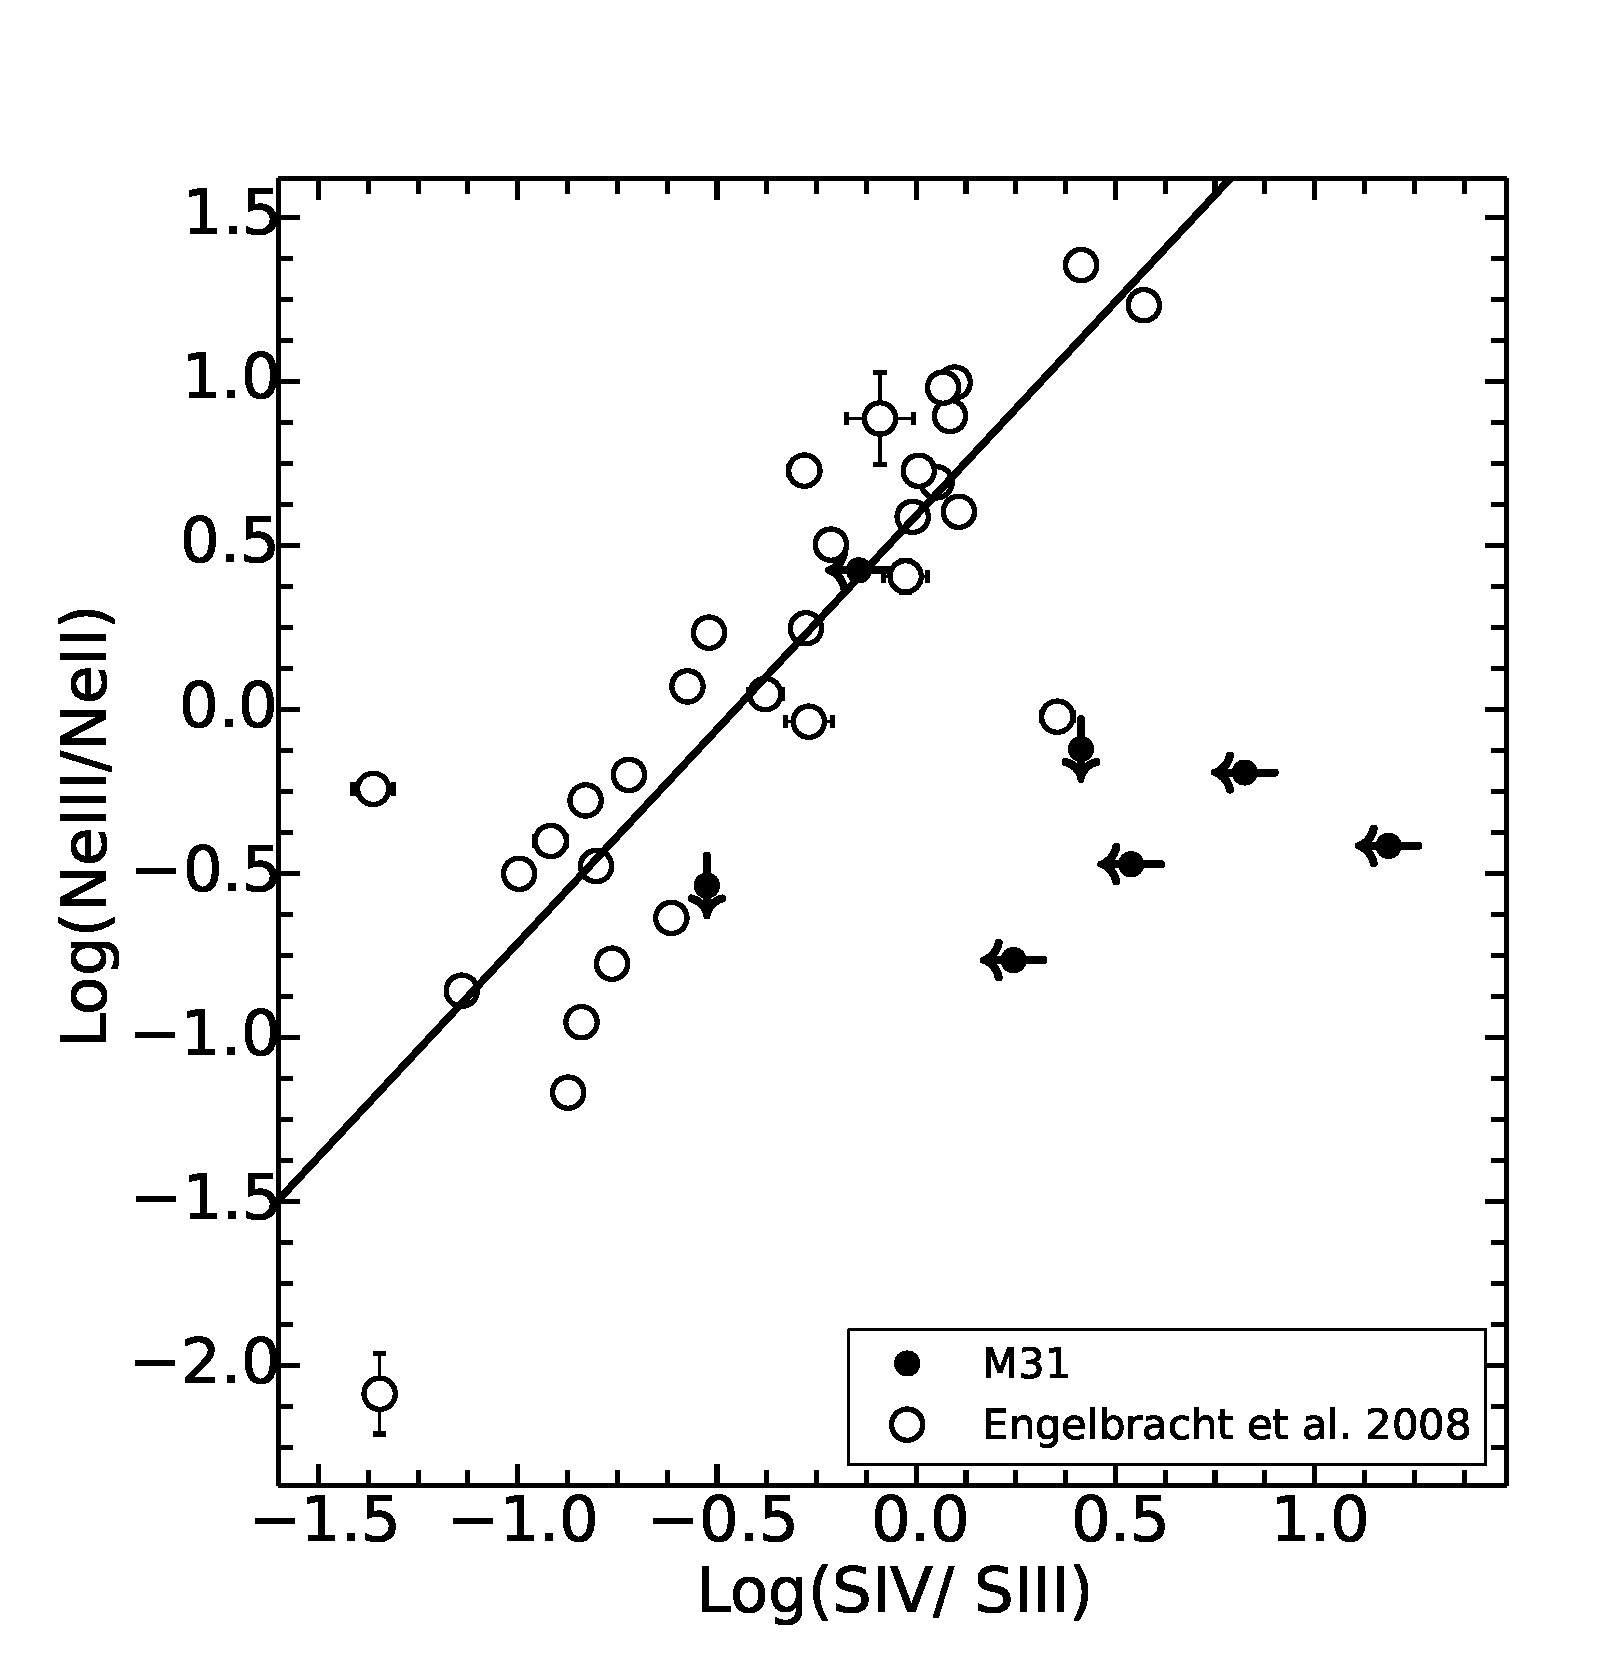
\includegraphics[scale=0.3]{./NevsS.eps}
\caption{ Log([Ne~{\sc iii}]/[Ne~{\sc ii}])  vs Log([S~{\sc iv}]/[S~{\sc iii}]) 18 for the M31 regions in our sample (black dots) and for the starburst sample from \citet{Engelbracht_2008} (open dots). The straight line is the line of best fit for the starburst sample.}
\label{SvsNe}
\end{figure}

%SPW: Sec 3.4: this is much too long for basically no result.  Unless I'm missing something, the key point is that all the regions are relatively low excitation.  In the one possible exception (6), the [Ne III] flux is based on only a single data point.  I think Table 4 and Fig 10 are fine, but the discussion can be a paragraph.
%MLNA: Does PAHFIT *separately* fit an independent Gaussian to each of the atomic lines in Sec 3.4?  They are not correlated in any way?
PAHFIT also returns the emission line strengths and the flux uncertainties of atomic lines. These are listed in Table~\ref{Atomic}.
Line ratios of [Ne~{\sc iii}]/[Ne~{\sc ii}] and [S~{\sc iv}]/[S~{\sc iii}] 18 have been used as an indication of the radiation hardness. \citet{Engelbracht_2008} demonstrated that a combination of these two line ratios -which they call the radiation hardness index (RHI)- is a more sensitive indicator of the hardness of the radiation. The RHI values are calculated using
\begin{equation}
{\rm RHI} = \left( \log\frac{\textrm{[Ne~{\sc iii}] }}{\textrm{[Ne~{\sc ii}]}} + [0.71 + 1.58\log\frac{\textrm{{[S~{\sc iv}]}}}{\textrm{{[S~{\sc iv}]}}}\right) /2
\end{equation}
Here, 1.58 and 0.71 are the slope and the intercept of the [Ne~{\sc iii}]/[Ne~{\sc ii}]  vs [S~{\sc iv}]/[S~{\sc iii}] 18 plot (Figure \ref{SvsNe}) for the starburst sample from 
\citet{Engelbracht_2008}. The RHI has also been used by \citet{Gordon:2008lr} for M101 observations. To investigate whether the atomic line emission from the selected regions of M31 with the fit parameters described above, we compared them to the starburst sample (Figure \ref{SvsNe}). 
	
We calculated upper limits for non-detected lines \footnote{To find the upper limits for the flux of missing atomic lines, we assumed the line to be a 
Gaussian profile with a FWHM as given by PAHFIT. The peak intensity was taken to be 3 times the RMS, where RMS is the root mean square of 
the noise at the position of a missing line.}. Figure \ref{SvsNe}  shows that the limits are reasonably following the trend for the starburst galaxy sample. 
Therefore the equation mentioned above was adopted with a simple modification to calculate the RHI values for our sample. For the regions with missing Ne lines, 
equation~\ref{eq:s} was used and for the regions with missing S lines, equation~\ref{eq:ne} was used. 
\begin{equation}
{\rm RHI} = 0.71 + 1.58\log\frac{\textrm{[S~{\sc iv}]}}{\textrm{[S~{\sc iii}]}}
\label{eq:s}	
\end{equation}
\begin{equation}
{\rm RHI} = \log\frac{\textrm{[Ne~{\sc iii}]}}{\textrm{[Ne~{\sc ii}]}}
\label{eq:ne}	
\end{equation}
For Regions 2, 5, and 8, we used the upper limit values of their atomic line intensities to calculated RHI values.
